\section{设计步骤}

\subsection{初始结构的选择}

初始结构的选取是光学设计流程中的关键环节。对于由多片透镜组成的目视系统而言，评价函数优化本质上是在已有结构附近进行参数搜索；若初始结构的光焦度分配、光阑位置、玻璃组合和空气间隔不合理，优化算法容易陷入局部极值，甚至出现负厚度、边缘过薄或光线截断等非物理解。因此，初始结构不应简单理解为一组可任意调整的几何参数，而应是满足近轴成像关系、基本像差校正规律和加工约束的“可优化起点”\cite{Kingslake2010,Fischer2008,Laikin2007}。

凯尔纳目镜属于经典三片式目镜，其结构自由度有限，但场镜、消色差双合镜和空气间隔之间存在明确的像差分工。初始结构的获取通常可采用以下几类较为规范的方法：

\begin{itemize}
\item
  经典结构缩放法：以光学设计教材、镜头设计手册或成熟设计实例中的凯尔纳目镜为母型，保持透镜面序、玻璃类型和相对厚度关系不变，根据目标有效焦距进行等比例缩放。该方法的理论基础是近轴光学的一阶比例关系：在相同折射率和相似结构下，曲率半径、厚度和空气间隔可随焦距按比例放大或缩小，而相对像差分布能够在一定范围内保持相似。因此，该方法适合用于结构明确、目标焦距变化不大的经典系统。
\item
  文献与专利反演法：从公开论文、专利和光学设计数据库中选取与目标焦距、视场角、孔径和镜片数量相近的目镜结构，提取其曲率半径、厚度、玻璃材料和光阑位置作为初始数据，再通过焦距归一化和孔径匹配建立模型。该方法的优点是初始像差水平通常较低，适用于工程设计中快速获得可收敛结构；不足是需要对公开结构的工作波长、视场定义、孔径类型和像面位置进行严格核对，避免直接套用造成指标不一致。
\item
  像差理论综合法：从近轴光线追迹和三级像差理论出发，先确定系统总光焦度、场镜与目镜组的光焦度分配，再根据消色差条件选择冕牌/火石玻璃组合，并利用弯曲因子、空气间隔和光阑位置初步平衡球差、彗差、像散、场曲和畸变。该方法理论性较强，能够解释结构参数对像差的影响规律，但计算量较大，通常需要与光学设计软件的逐步优化结合使用。
\item
  混合优化起点法：先采用经典结构缩放或文献结构作为一阶起点，再利用近轴约束和像差分析对关键变量进行预调整，例如控制场镜弯曲方向、胶合组曲率分配、后焦距和边缘光线高度。该方法兼具经验结构的稳定性和理论校正的针对性，是实际镜头设计中较常用的工作方式。
\end{itemize}

综合本设计的任务特点，系统要求为中等焦距、中等视场且镜片数量限定为凯尔纳目镜的基本三片结构，因此采用“经典结构缩放法”为主、“混合优化起点法”为辅的策略。具体做法是：首先选取经典凯尔纳目镜结构作为母型，保持场镜加消色差双合镜的基本面序；其次在Zemax中通过Scale Lens功能将有效焦距调整到30 mm附近；然后结合入瞳直径、半视场角、有效半口径和机械半口径要求，对光阑位置、空气间隔和各面口径进行检查，为后续Merit Function优化提供稳定的起始模型\cite{Yu2016,Geary2002,Laikin2007,Zemax2021}。初始结构的镜头数据如下表所示：

表3.1 系统初始结构（Lens Data）

\begin{longtable}[]{@{}
  >{\raggedright\arraybackslash}p{(\columnwidth - 14\tabcolsep) * \real{0.0700}}
  >{\raggedright\arraybackslash}p{(\columnwidth - 14\tabcolsep) * \real{0.1250}}
  >{\raggedright\arraybackslash}p{(\columnwidth - 14\tabcolsep) * \real{0.1450}}
  >{\raggedright\arraybackslash}p{(\columnwidth - 14\tabcolsep) * \real{0.1250}}
  >{\raggedright\arraybackslash}p{(\columnwidth - 14\tabcolsep) * \real{0.1000}}
  >{\raggedright\arraybackslash}p{(\columnwidth - 14\tabcolsep) * \real{0.1450}}
  >{\raggedright\arraybackslash}p{(\columnwidth - 14\tabcolsep) * \real{0.1450}}
  >{\raggedright\arraybackslash}p{(\columnwidth - 14\tabcolsep) * \real{0.1450}}@{}}
\toprule\noalign{}
\endhead
\bottomrule\noalign{}
\endlastfoot
\textbf{面号} & \textbf{面型} & \textbf{曲率半径 R (mm)} & \textbf{厚度 T (mm)} & \textbf{玻璃材料} & \textbf{有效半口径 (mm)} & \textbf{机械半口径 (mm)} & \textbf{备注} \\
OBJ & 标准面 & Infinity & Infinity & --- & Infinity & Infinity & 物面 \\
1 & 标准面 & Infinity & 5.100 & --- & 2.000 & 2.000 & STOP，光阑面 \\
2 & 标准面 & 153.000 & 2.000 & F4 & 4.136 & 6.401 & 第一片透镜前表面 \\
3 & 标准面 & 14.900 & 8.000 & BAK2 & 4.770 & 6.401 & 第一片透镜后表面 \\
4 & 标准面 & −19.900 & 22.300 & --- & 6.401 & 6.401 & 空气间隔 \\
5 & 标准面 & 23.500 & 6.000 & BAK2 & 12.481 & 12.481 & 第二片透镜前表面 \\
6 & 标准面 & Infinity & 7.710 & --- & 12.278 & 12.481 & 第二片透镜后表面 \\
IMA & 标准面 & Infinity & --- & --- & 11.278 & 11.278 & 像面 \\
\end{longtable}

\subsubsection{Zemax建模步骤}

在Zemax OpticStudio中建立初始模型的具体步骤如下：

\begin{enumerate}
\def\labelenumi{\arabic{enumi}.}
\item
  新建Sequential模式工程，在System Explorer中设置孔径类型为入瞳直径（Entrance Pupil Diameter），数值设为4 mm；
\item
  在Fields（视场）选项中设置5个归一化视场：0、0.25、0.50、0.75、1.00，对应轴上到\(\pm 22.5^\circ\)全视场的不同观测方向；
\item
  在Wavelengths（波长）中添加三个工作波长：587.6 nm（d光，权重1，主波长）、486.1 nm（F光，权重1）、656.3 nm（C光，权重1）；
\item
  在Lens Data Editor中依次录入各面的曲率半径、厚度和玻璃材料（F4、BAK2），并设置各面的有效半口径与机械半口径；
\item
  通过System Data菜单确认有效焦距（EFL）是否约为30 mm，若偏差较大，使用Scale Lens功能整体缩放；
\item
  在Layout分析窗口查看2D光路图，确认光线走向正确，无全内反射或光线截断等异常情况。
\end{enumerate}

\begin{figure}[H]
  \centering
  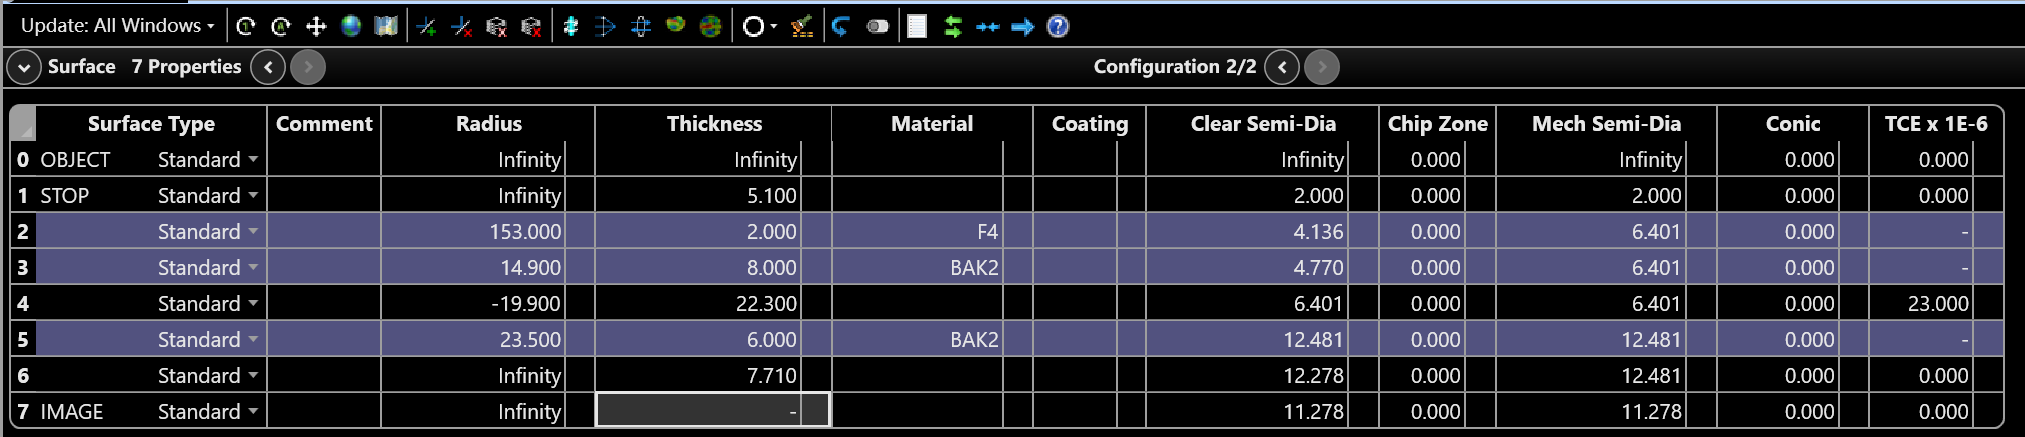
\includegraphics[width=0.95\textwidth]{chapters/chapter3/figures/lens_data.png}
  \caption{Zemax初始结构Lens Data Editor界面}
  \label{fig:lens-data}
\end{figure}

\subsection{手动修改参数}

由于初始结构来源于教材，直接按比例缩放后可能存在以下问题，需要在进行自动优化之前手动修改部分参数：

\begin{enumerate}
\def\labelenumi{\arabic{enumi}.}
\item
  场曲偏大：初始结构的切向和弧矢焦面存在分离，需要微调场镜曲率半径，利用场镜弯月形状引入反向场曲进行预校正；
\item
  出瞳距离不足：若自动求解后出瞳位置不满足\(\ge\)10 mm要求，需调整场镜与双合镜之间的空气间隔；
\item
  全内反射风险：在较大视场角下，某些面（尤其是场镜后表面）可能出现全反射，需检查各面的入射角是否超过临界角，必要时适当增大该面的曲率半径；
\item
  相对照度过低：全视场的相对照度若低于80\%，说明存在渐晕，需调整光阑位置或透镜口径。
\end{enumerate}

手动调整的重点是面2（场镜后表面曲率半径）和面3（空气间隔）这两个参数，通过在Zemax中实时观察像差曲线和系统数据，逐步将系统调整到接近设计要求的初始状态，然后再进行自动优化。

\subsection{设置优化函数}

在Zemax的Merit Function Editor中进行评价函数设置，是自动优化前的关键步骤。评价函数的设置直接决定了优化的方向和最终结果的质量\cite{Fischer2008,Laikin2007,Zemax2021}。

对于本次凯尔纳目镜设计，优化评价函数直接参考优化向导文件\verb|osd.MF|设置。该文件以RMS spot x+y centroid为核心评价指标，并叠加焦距、光程和厚度边界约束。具体设置策略如下：

\begin{itemize}
\item
  焦距与系统尺度控制：使用EFFL将系统有效焦距控制为30 mm；使用TOTR作为系统长度监控量，优化向导记录值约为46.197 mm；同时保留OPLT=60和OPGT=7两个光程相关辅助约束；
\item
  像质约束：采用Zemax优化向导生成的RMS spot x+y centroid评价函数，通过TRCX和TRCY操作数分别约束各采样光线在质心参考下的X、Y方向横向像差；
\item
  视场均衡：对0、0.25、0.50、0.75、1.00五个归一化视场进行采样，覆盖轴上到全视场，避免只优化轴上或边缘视场导致中间视场像质失衡；
\item
  可加工性约束：对各面加入MNCA、MXCA、MNEA、MNCG、MXCG、MNEG等厚度边界操作数，限制空气间隔、玻璃中心厚度和玻璃边缘厚度，防止优化过程中出现负厚度、过薄边缘或过厚镜片。
\end{itemize}

表3.2 Merit Function主要操作数设置

\begin{longtable}[]{@{}
  >{\raggedright\arraybackslash}p{(\columnwidth - 8\tabcolsep) * \real{0.1662}}
  >{\raggedright\arraybackslash}p{(\columnwidth - 8\tabcolsep) * \real{0.3353}}
  >{\raggedright\arraybackslash}p{(\columnwidth - 8\tabcolsep) * \real{0.1773}}
  >{\raggedright\arraybackslash}p{(\columnwidth - 8\tabcolsep) * \real{0.1551}}
  >{\raggedright\arraybackslash}p{(\columnwidth - 8\tabcolsep) * \real{0.1662}}@{}}
\toprule\noalign{}
\endhead
\bottomrule\noalign{}
\endlastfoot
\textbf{操作数} & \textbf{含义} & \textbf{目标值} & \textbf{权重} & \textbf{备注} \\
EFFL & 系统有效焦距 & 30 mm & 1 & 实际值约30.000004 mm \\
TOTR & 系统长度监控 & 约46.197 mm & -- & Merit Function中的监控量，最终几何厚度见第5章 \\
OPLT & 光程相关约束 & 60 & 1 & 用于稳定优化过程 \\
OPGT & 光程/结构相关约束 & 7 & 1 & 用于稳定优化过程 \\
DMFS & 默认评价函数说明 & RMS spot x+y centroid & -- & X、Y权重均为1，GQ采样3环6臂 \\
TRCX/\newline TRCY & 横向像差操作数 & 最小化 & 自动生成 & 覆盖5个视场、3个波长及瞳面采样点 \\
MNCA/\newline MNEA & 空气中心/边缘厚度下限 & \(\ge\)0.3 mm & 1 & 第6面边缘空气约束为5.0 mm \\
MNCG/\newline MNEG & 玻璃中心/边缘厚度下限 & \(\ge\)1.0 mm & 1 & 保证镜片可加工性 \\
MXCG & 玻璃中心厚度上限 & \(\le\)6.0 mm & 1 & 控制镜片厚度 \\
MXCA & 空气中心厚度上限 & \(\le\)1000 mm & 1 & 宽松边界，防止异常发散 \\
\end{longtable}

因此，本设计的优化重点并不是单独使用畸变或波前误差操作数，而是在保持30 mm有效焦距和合理结构尺寸的前提下，使5个视场的RMS点列半径整体下降。畸变、场曲和色差等像差指标在后续分析章节中通过相应图表进行检验。
